\documentclass{standalone}
\usepackage{tikz}
\usetikzlibrary{patterns, positioning}

\begin{document}
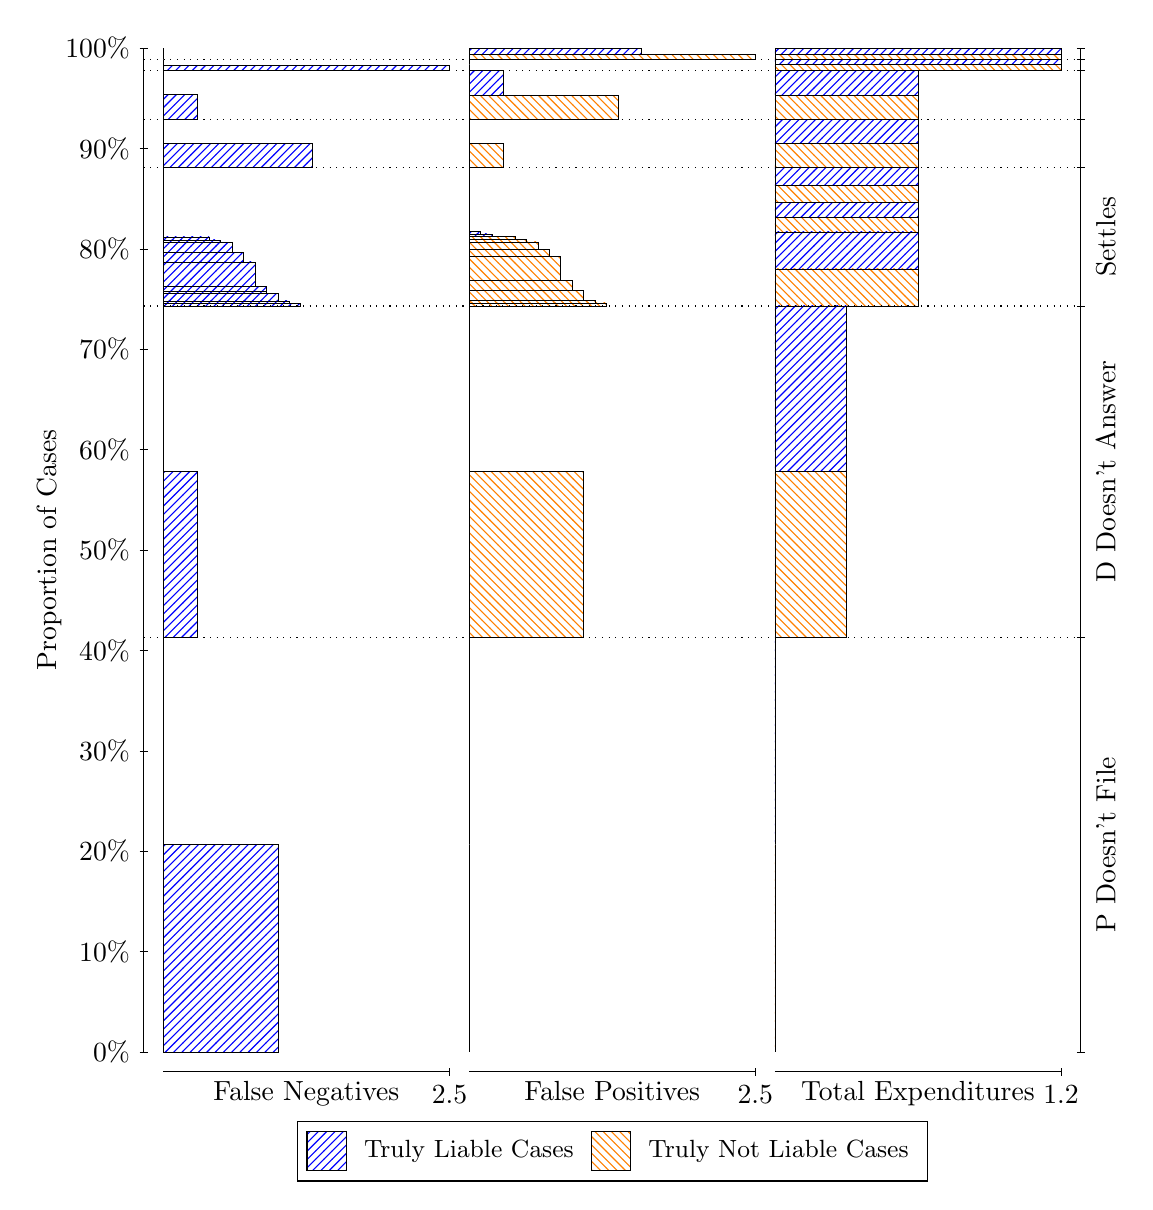
\begin{tikzpicture}
\draw[black, very thin] (1.5,1.75) -- (1.5,14.5);
\node[rotate=90, anchor=center] at (0.3, 8.125) {Proportion of Cases};
\draw[black, very thin] (1.45,1.75) -- (1.55,1.75);
\node[anchor=east] at (1.45, 1.75) {0\%};
\draw[black, very thin] (1.45,3.025) -- (1.55,3.025);
\node[anchor=east] at (1.45, 3.025) {10\%};
\draw[black, very thin] (1.45,4.3) -- (1.55,4.3);
\node[anchor=east] at (1.45, 4.3) {20\%};
\draw[black, very thin] (1.45,5.575) -- (1.55,5.575);
\node[anchor=east] at (1.45, 5.575) {30\%};
\draw[black, very thin] (1.45,6.85) -- (1.55,6.85);
\node[anchor=east] at (1.45, 6.85) {40\%};
\draw[black, very thin] (1.45,8.125) -- (1.55,8.125);
\node[anchor=east] at (1.45, 8.125) {50\%};
\draw[black, very thin] (1.45,9.4) -- (1.55,9.4);
\node[anchor=east] at (1.45, 9.4) {60\%};
\draw[black, very thin] (1.45,10.675) -- (1.55,10.675);
\node[anchor=east] at (1.45, 10.675) {70\%};
\draw[black, very thin] (1.45,11.95) -- (1.55,11.95);
\node[anchor=east] at (1.45, 11.95) {80\%};
\draw[black, very thin] (1.45,13.225) -- (1.55,13.225);
\node[anchor=east] at (1.45, 13.225) {90\%};
\draw[black, very thin] (1.45,14.5) -- (1.55,14.5);
\node[anchor=east] at (1.45, 14.5) {100\%};

\draw[black, very thin] (13.4,1.75) -- (13.4,14.5);
\draw[black, very thin] (13.35,1.75) -- (13.45,1.75);
\node[anchor=west] at (13.35, 1.75) {};
\draw[black, very thin] (13.35,7.0156) -- (13.45,7.0156);
\node[anchor=west] at (13.35, 7.0156) {};
\draw[black, very thin] (13.35,11.224) -- (13.45,11.224);
\node[anchor=west] at (13.35, 11.224) {};
\draw[black, very thin] (13.35,12.981) -- (13.45,12.981);
\node[anchor=west] at (13.35, 12.981) {};
\draw[black, very thin] (13.35,13.597) -- (13.45,13.597);
\node[anchor=west] at (13.35, 13.597) {};
\draw[black, very thin] (13.35,14.214) -- (13.45,14.214);
\node[anchor=west] at (13.35, 14.214) {};
\draw[black, very thin] (13.35,14.357) -- (13.45,14.357);
\node[anchor=west] at (13.35, 14.357) {};
\draw[black, very thin] (13.35,14.5) -- (13.45,14.5);
\node[anchor=west] at (13.35, 14.5) {};

\draw[black, very thin, pattern color=blue, pattern=north east lines] (1.75,1.75) rectangle (3.2033,4.3828);
\draw[black, very thin, pattern color=orange, pattern=north west lines] (1.75,4.3828) rectangle (1.75,7.0156);
\draw[black, very thin, pattern color=blue, pattern=north east lines] (1.75,7.0156) rectangle (2.186,9.12);
\draw[black, very thin, pattern color=orange, pattern=north west lines] (1.75,9.12) rectangle (1.75,11.224);
\draw[black, very thin, pattern color=blue, pattern=north east lines] (1.75,11.224) rectangle (3.494,11.258);
\draw[black, very thin, pattern color=blue, pattern=north east lines] (1.75,11.258) rectangle (3.3487,11.29);
\draw[black, very thin, pattern color=blue, pattern=north east lines] (1.75,11.29) rectangle (3.2033,11.387);
\draw[black, very thin, pattern color=blue, pattern=north east lines] (1.75,11.387) rectangle (3.058,11.41);
\draw[black, very thin, pattern color=blue, pattern=north east lines] (1.75,11.41) rectangle (3.058,11.475);
\draw[black, very thin, pattern color=blue, pattern=north east lines] (1.75,11.475) rectangle (2.9127,11.783);
\draw[black, very thin, pattern color=blue, pattern=north east lines] (1.75,11.783) rectangle (2.7673,11.901);
\draw[black, very thin, pattern color=blue, pattern=north east lines] (1.75,11.901) rectangle (2.622,12.029);
\draw[black, very thin, pattern color=blue, pattern=north east lines] (1.75,12.029) rectangle (2.4767,12.064);
\draw[black, very thin, pattern color=blue, pattern=north east lines] (1.75,12.064) rectangle (2.3313,12.102);
\draw[black, very thin, pattern color=orange, pattern=north west lines] (1.75,12.102) rectangle (1.75,12.981);
\draw[black, very thin, pattern color=blue, pattern=north east lines] (1.75,12.981) rectangle (3.6393,13.285);
\draw[black, very thin, pattern color=orange, pattern=north west lines] (1.75,13.285) rectangle (1.75,13.597);
\draw[black, very thin, pattern color=blue, pattern=north east lines] (1.75,13.597) rectangle (2.186,13.91);
\draw[black, very thin, pattern color=orange, pattern=north west lines] (1.75,13.91) rectangle (1.75,14.214);
\draw[black, very thin, pattern color=blue, pattern=north east lines] (1.75,14.214) rectangle (5.3833,14.28);
\draw[black, very thin, pattern color=orange, pattern=north west lines] (1.75,14.28) rectangle (1.75,14.357);
\draw[black, very thin, pattern color=orange, pattern=north west lines] (1.75,14.357) rectangle (1.75,14.422);
\draw[black, very thin, pattern color=blue, pattern=north east lines] (1.75,14.422) rectangle (1.75,14.5);
\draw[black, very thin, pattern color=orange, pattern=north west lines] (5.6333,1.75) rectangle (5.6333,4.3828);
\draw[black, very thin, pattern color=blue, pattern=north east lines] (5.6333,4.3828) rectangle (5.6333,7.0156);
\draw[black, very thin, pattern color=orange, pattern=north west lines] (5.6333,7.0156) rectangle (7.0867,9.12);
\draw[black, very thin, pattern color=blue, pattern=north east lines] (5.6333,9.12) rectangle (5.6333,11.224);
\draw[black, very thin, pattern color=orange, pattern=north west lines] (5.6333,11.224) rectangle (7.3773,11.263);
\draw[black, very thin, pattern color=orange, pattern=north west lines] (5.6333,11.263) rectangle (7.232,11.296);
\draw[black, very thin, pattern color=orange, pattern=north west lines] (5.6333,11.296) rectangle (7.0867,11.425);
\draw[black, very thin, pattern color=orange, pattern=north west lines] (5.6333,11.425) rectangle (6.9413,11.545);
\draw[black, very thin, pattern color=orange, pattern=north west lines] (5.6333,11.545) rectangle (6.796,11.854);
\draw[black, very thin, pattern color=orange, pattern=north west lines] (5.6333,11.854) rectangle (6.6507,11.941);
\draw[black, very thin, pattern color=orange, pattern=north west lines] (5.6333,11.941) rectangle (6.5053,12.037);
\draw[black, very thin, pattern color=orange, pattern=north west lines] (5.6333,12.037) rectangle (6.36,12.07);
\draw[black, very thin, pattern color=orange, pattern=north west lines] (5.6333,12.07) rectangle (6.2147,12.103);
\draw[black, very thin, pattern color=blue, pattern=north east lines] (5.6333,12.103) rectangle (5.924,12.141);
\draw[black, very thin, pattern color=blue, pattern=north east lines] (5.6333,12.141) rectangle (5.7787,12.176);
\draw[black, very thin, pattern color=blue, pattern=north east lines] (5.6333,12.176) rectangle (5.6333,12.981);
\draw[black, very thin, pattern color=orange, pattern=north west lines] (5.6333,12.981) rectangle (6.0693,13.293);
\draw[black, very thin, pattern color=blue, pattern=north east lines] (5.6333,13.293) rectangle (5.6333,13.597);
\draw[black, very thin, pattern color=orange, pattern=north west lines] (5.6333,13.597) rectangle (7.5227,13.902);
\draw[black, very thin, pattern color=blue, pattern=north east lines] (5.6333,13.902) rectangle (6.0693,14.214);
\draw[black, very thin, pattern color=orange, pattern=north west lines] (5.6333,14.214) rectangle (5.6333,14.291);
\draw[black, very thin, pattern color=blue, pattern=north east lines] (5.6333,14.291) rectangle (5.6333,14.357);
\draw[black, very thin, pattern color=orange, pattern=north west lines] (5.6333,14.357) rectangle (9.2667,14.422);
\draw[black, very thin, pattern color=blue, pattern=north east lines] (5.6333,14.422) rectangle (7.8133,14.5);
\draw[black, very thin, pattern color=orange, pattern=north west lines] (9.5167,1.75) rectangle (9.5167,4.3828);
\draw[black, very thin, pattern color=blue, pattern=north east lines] (9.5167,4.3828) rectangle (9.5167,7.0156);
\draw[black, very thin, pattern color=orange, pattern=north west lines] (9.5167,7.0156) rectangle (10.425,9.12);
\draw[black, very thin, pattern color=blue, pattern=north east lines] (9.5167,9.12) rectangle (10.425,11.224);
\draw[black, very thin, pattern color=orange, pattern=north west lines] (9.5167,11.224) rectangle (11.333,11.695);
\draw[black, very thin, pattern color=blue, pattern=north east lines] (9.5167,11.695) rectangle (11.333,12.166);
\draw[black, very thin, pattern color=orange, pattern=north west lines] (9.5167,12.166) rectangle (11.333,12.351);
\draw[black, very thin, pattern color=blue, pattern=north east lines] (9.5167,12.351) rectangle (11.333,12.536);
\draw[black, very thin, pattern color=orange, pattern=north west lines] (9.5167,12.536) rectangle (11.333,12.759);
\draw[black, very thin, pattern color=blue, pattern=north east lines] (9.5167,12.759) rectangle (11.333,12.981);
\draw[black, very thin, pattern color=orange, pattern=north west lines] (9.5167,12.981) rectangle (11.333,13.293);
\draw[black, very thin, pattern color=blue, pattern=north east lines] (9.5167,13.293) rectangle (11.333,13.597);
\draw[black, very thin, pattern color=orange, pattern=north west lines] (9.5167,13.597) rectangle (11.333,13.902);
\draw[black, very thin, pattern color=blue, pattern=north east lines] (9.5167,13.902) rectangle (11.333,14.214);
\draw[black, very thin, pattern color=orange, pattern=north west lines] (9.5167,14.214) rectangle (13.15,14.291);
\draw[black, very thin, pattern color=blue, pattern=north east lines] (9.5167,14.291) rectangle (13.15,14.357);
\draw[black, very thin, pattern color=orange, pattern=north west lines] (9.5167,14.357) rectangle (13.15,14.422);
\draw[black, very thin, pattern color=blue, pattern=north east lines] (9.5167,14.422) rectangle (13.15,14.5);
\draw[black, dotted] (1.5,7.0156) -- (13.4,7.0156);
\draw[black, dotted] (1.5,11.224) -- (13.4,11.224);
\draw[black, dotted] (1.5,12.981) -- (13.4,12.981);
\draw[black, dotted] (1.5,13.597) -- (13.4,13.597);
\draw[black, dotted] (1.5,14.214) -- (13.4,14.214);
\draw[black, dotted] (1.5,14.357) -- (13.4,14.357);
\draw[black, very thin] (1.75,1.5) -- (5.3833,1.5);
\node[anchor=north] at (3.5667, 1.5) {False Negatives};
\draw[black, very thin] (5.3833,1.45) -- (5.3833,1.55);
\node[anchor=north] at (5.3833, 1.45) {2.5};

\draw[black, very thin] (5.6333,1.5) -- (9.2667,1.5);
\node[anchor=north] at (7.45, 1.5) {False Positives};
\draw[black, very thin] (9.2667,1.45) -- (9.2667,1.55);
\node[anchor=north] at (9.2667, 1.45) {2.5};

\draw[black, very thin] (9.5167,1.5) -- (13.15,1.5);
\node[anchor=north] at (11.333, 1.5) {Total Expenditures};
\draw[black, very thin] (13.15,1.45) -- (13.15,1.55);
\node[anchor=north] at (13.15, 1.45) {1.2};

\node[black, centered, rotate=90] at (13.72, 4.3828) {P Doesn't File};
\node[black, centered, rotate=90] at (13.72, 9.12) {D Doesn't Answer};
\node[black, centered, rotate=90] at (13.72, 12.103) {Settles};





\draw (7.449999999999999,1.5) node[draw=none] (baseCoordinate) {};
\begin{scope}[align=center]
        \matrix[scale=0.5, draw=black, below=0.5cm of baseCoordinate, nodes={draw}, column sep=0.1cm]{
            \node[rectangle, draw, minimum width=0.5cm, minimum height=0.5cm, pattern=north east lines, pattern color=blue] {}; &
            \node[draw=none, font=\small] (B) {Truly Liable Cases}; &
            \node[rectangle, draw, minimum width=0.5cm, minimum height=0.5cm, pattern=north west lines, pattern color=orange] {}; &
            \node[draw=none, font=\small] (B) {Truly Not Liable Cases}; \\
            };
\end{scope}

\end{tikzpicture}
\end{document}